%%%%%%%%%%%%%%%%%%%%%%%%%%%%%%%%%%%%%%%%%%%%%%%%%%%%%%%%%%%%%%%%%%%%%%%%%%%%%
% chapters/chapter-3.tex
%%%%%%%%%%%%%%%%%%%%%%%%%%%%%%%%%%%%%%%%%%%%%%%%%%%%%%%%%%%%%%%%%%%%%%%%%%%%%

\chapter{The ATLAS experiment at the Large Hadron Collider}
\label{chap:atlas}

\section{The Large Hadron Collider}

The Large Hadron Collider (LHC) is the world's largest and most powerful particle accelerator, located at the European Organization for Nuclear Research (CERN) near Geneva, in Switzerland. The LHC is installed in the 26.7 km circumference tunnel that previously housed the Large Electron-Positron Collider (LEP) and collides beams of protons and heavy ions at the highest energies ever achieved to enable the exploration of fundamental physics on the TeV scale.

\subsection{Accelerator Complex}

The LHC is the final stage in CERN's accelerator complex. Before reaching the main ring, particles are first accelerated to high energies by a series of smaller machines. The acceleration chain for protons is illustrated in Figure~\ref{fig:cernaccelerators} and includes the following stages:

\begin{enumerate}
\item \textbf{Proton source:} Hydrogen gas is ionized to produce protons, which are initially accelerated to 750 keV by a radio-frequency quadrupole.

\item \textbf{LINAC 4:} The linear accelerator boosts protons to 160 MeV using radio-frequency cavities along a 90-meter straight section.

\item \textbf{Proton Synchrotron Booster (PSB):} Four superimposed rings accelerate protons to 2 GeV, increasing beam intensity through bunch compression.

\item \textbf{Proton Synchrotron (PS):} This 628-meter circumference synchrotron, operational since 1959, accelerates protons to 26 GeV and performs bunch splitting to create the LHC bunch structure.

\item \textbf{Super Proton Synchrotron (SPS):} The 6.9 km circumference SPS serves as the final injector, accelerating protons to 450 GeV before transfer to the LHC.

\item \textbf{Large Hadron Collider:} Two counter-rotating beams are accelerated from 450 GeV injection energy to the operational beam energy, which has reached 6.8 TeV per beam (13.6 TeV center-of-mass energy) in Run 3, up from 6.5 TeV per beam (13 TeV collision energy) in Run 2.
\end{enumerate}

\begin{figure}[!htb]
\begin{center}
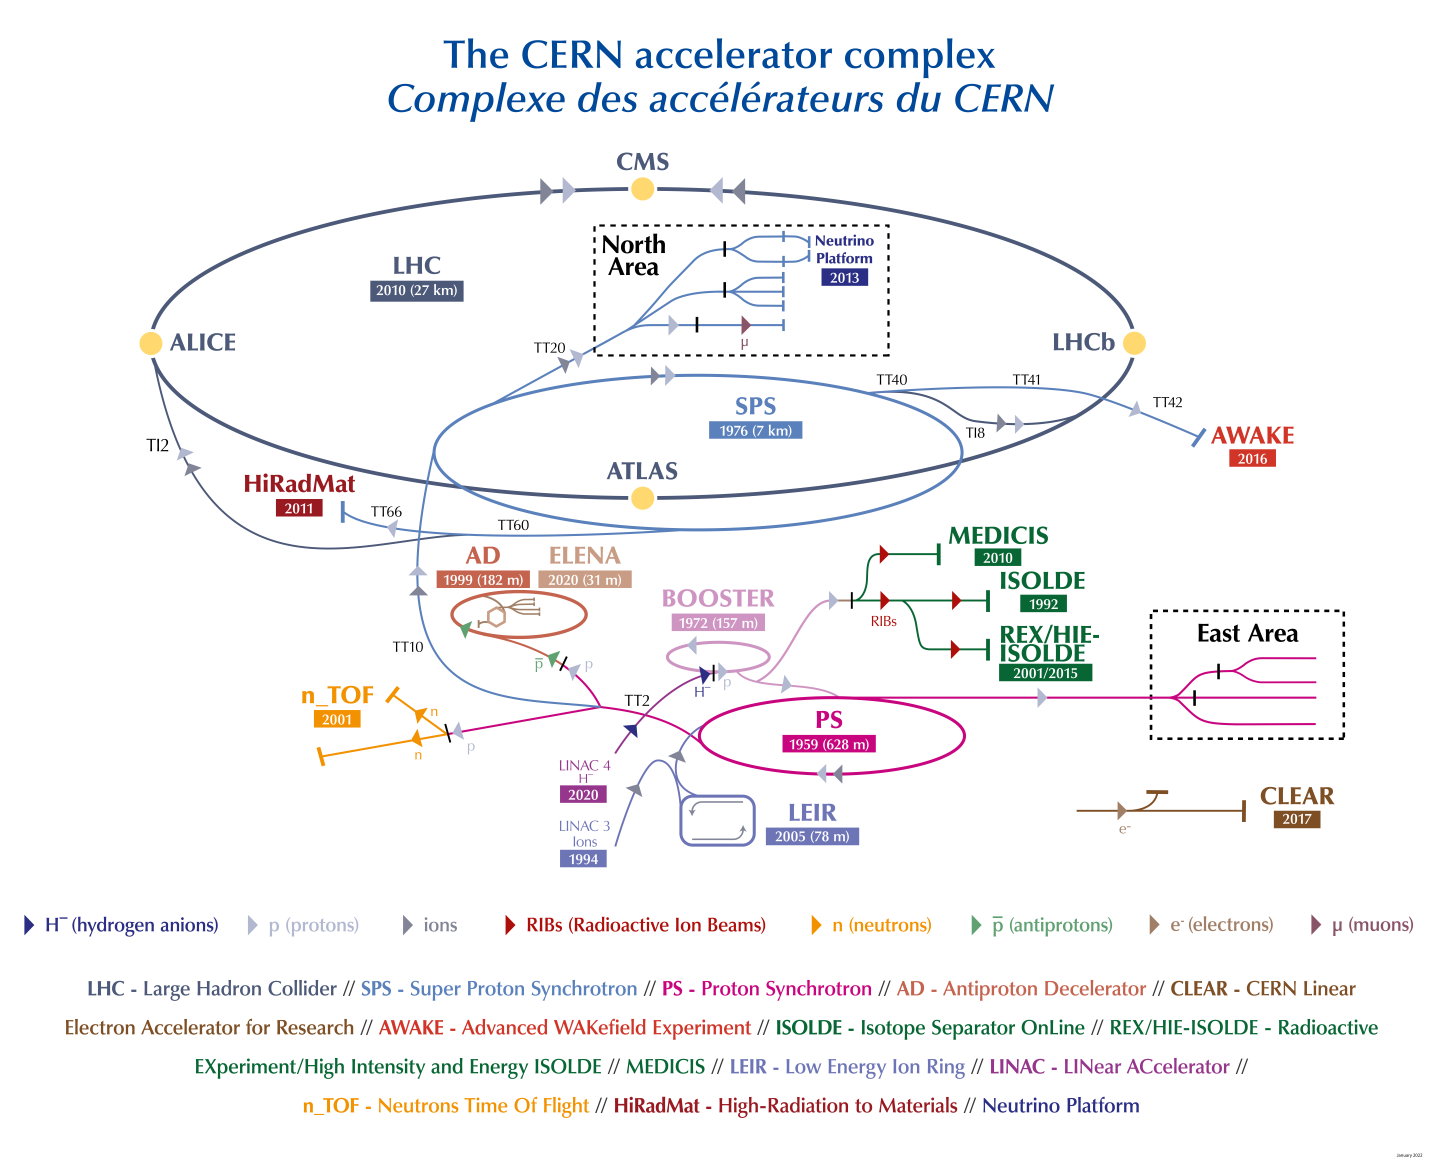
\includegraphics[width=0.8\textwidth]{figures/CCC-v2022.png}\caption{Schematic overview of the CERN accelerator complex.}
\label{fig:cernaccelerators}
\end{center}
\end{figure}

The LHC employs superconducting magnets to bend and focus the particle beams. The machine's 1232 main dipole magnets, each 15 meters in length, operate at 1.9 K using superfluid helium to generate magnetic fields of up to 8.33 T for beam bending. Meanwhile, 392 main quadrupole magnets are used to focus the beams. For acceleration, the RF system utilizes 400 MHz superconducting cavities to provide an energy boost of 16 MV per turn. To ensure the particles don't collide with stray gas molecules, an ultra-high vacuum of $10^{-13}$ atmospheres is maintained.

The beams are organized in a bunch structure, with up to 2808 bunches per beam separated by 25 ns (corresponding to 7.5 m spacing). Each bunch contains approximately $1.15 \times 10^{11}$ protons. The beam energy stored at full intensity reaches 362 MJ per beam, comparable to the kinetic energy of a 400-ton train at 150 km/h.

The LHC has operated at increasing center-of-mass energies: 7 TeV in 2010-2011, 8 TeV in 2012, 13 TeV during Run 2 (2015-2018), and currently 13.6 TeV in Run 3 (2022-2025), representing the highest collision energies ever achieved in a laboratory.

Four main experiments are installed at the LHC collision points: ATLAS (A Toroidal LHC ApparatuS) and CMS (Compact Muon Solenoid), general-purpose detectors designed to explore the full physics potential of the LHC and are located at Points 1 and 5 respectively; ALICE (A Large Ion Collider Experiment), located at Point 2 and specialized in heavy-ion collisions, studying the quark-gluon plasma formed in lead-lead collisions at $\sqrt{s_{NN}} = 5.02$ TeV per nucleon pair; LHCb (Large Hadron Collider beauty), optimized for b-physics, featuring a forward spectrometer designed to exploit the predominantly forward b-quark production in proton-proton collisions, located at Point 8.


\subsection{Luminosity}

Luminosity is a crucial measure of a particle collider's performance. It quantifies the number of collisions per unit time and area, and is therefore directly proportional to the event rate of any given physics process. The event rate for a physics process with cross-section $\sigma$ is given by:
\begin{equation}
R = \mathcal{L} \cdot \sigma,
\end{equation}
where $\mathcal{L}$ is the instantaneous luminosity, typically meaasured in units of cm$^{-2}$s$^{-1}$. For gaussian beams colliding head-on, the instantaneous luminosity can be approximated as:
\begin{equation}
\mathcal{L} = \frac{N_b^2 n_b f_{\text{rev}} \gamma}{4\pi \epsilon_n \beta^*} F,
\end{equation}
where $N_b$ is the number of particles per bunch, $n_b$ is the number of bunches, $f_{\text{rev}} $ is the revolution frequency, $\gamma$ is the Lorentz factor, $\epsilon_n$ is the normalized transverse emittance, $\beta^*$ is the beta function at the interaction point, and $F$ is a geometric factor accounting for the crossing angle. 

To determine the total number of events, $N$, for a process with cross-section $\sigma$ over a given period of time, one must use the integrated luminosity, $\mathcal{L}_\text{int}=\int \mathcal{L} \,dt$:
\begin{equation}
N = \mathcal{L}_\textbf{int} \cdot \sigma.
\end{equation}
The integrated luminosity is typically measured in units of inverse femtobarns (fb$^{-1}$), with 1 fb$^{-1}$ equivalent to 10$^{39}$ cm$^{-2}$.

As of 2025, the LHC Run 3 achieved peak instantaneous luminosities exceeding $2.0 \times 10^{34}$ cm$^{-2}$s$^{-1}$, with ATLAS and CMS each collecting over 100 fb$^{-1}$ of integrated luminosity. Run 3 is scheduled to continue through 2025, with a target of delivering approximately 300 fb$^{-1}$ to each general-purpose experiment.

The High-Luminosity LHC (HL-LHC) upgrade, scheduled to begin operations around 2029, will increase the integrated luminosity by a factor of 10, collecting up to 3000 fb$^{-1}$. This will enable percent-level measurements of Higgs couplings and significantly extend the mass reach for new particle searches.

\section{The ATLAS Experiment}

The ATLAS detector is a general-purpose particle detector at the LHC. Its main goal is to study the fudamental nature of the universe by precisely measuring the properties of particles that are created in high-energy proton-proton collisions. ATLAS is the largest volume particle detector ever constructed, measuring 44 meters in length and 25 meters in diameter, with a total weight of approximately 7000 tons. The detector consists of multiple subsystems arranged in concentric layers around the interaction point, as shown in Figure~\ref{fig:atlas_detector}, each optimized for measuring specific particle properties.

\begin{figure}[!htb]
\begin{center}
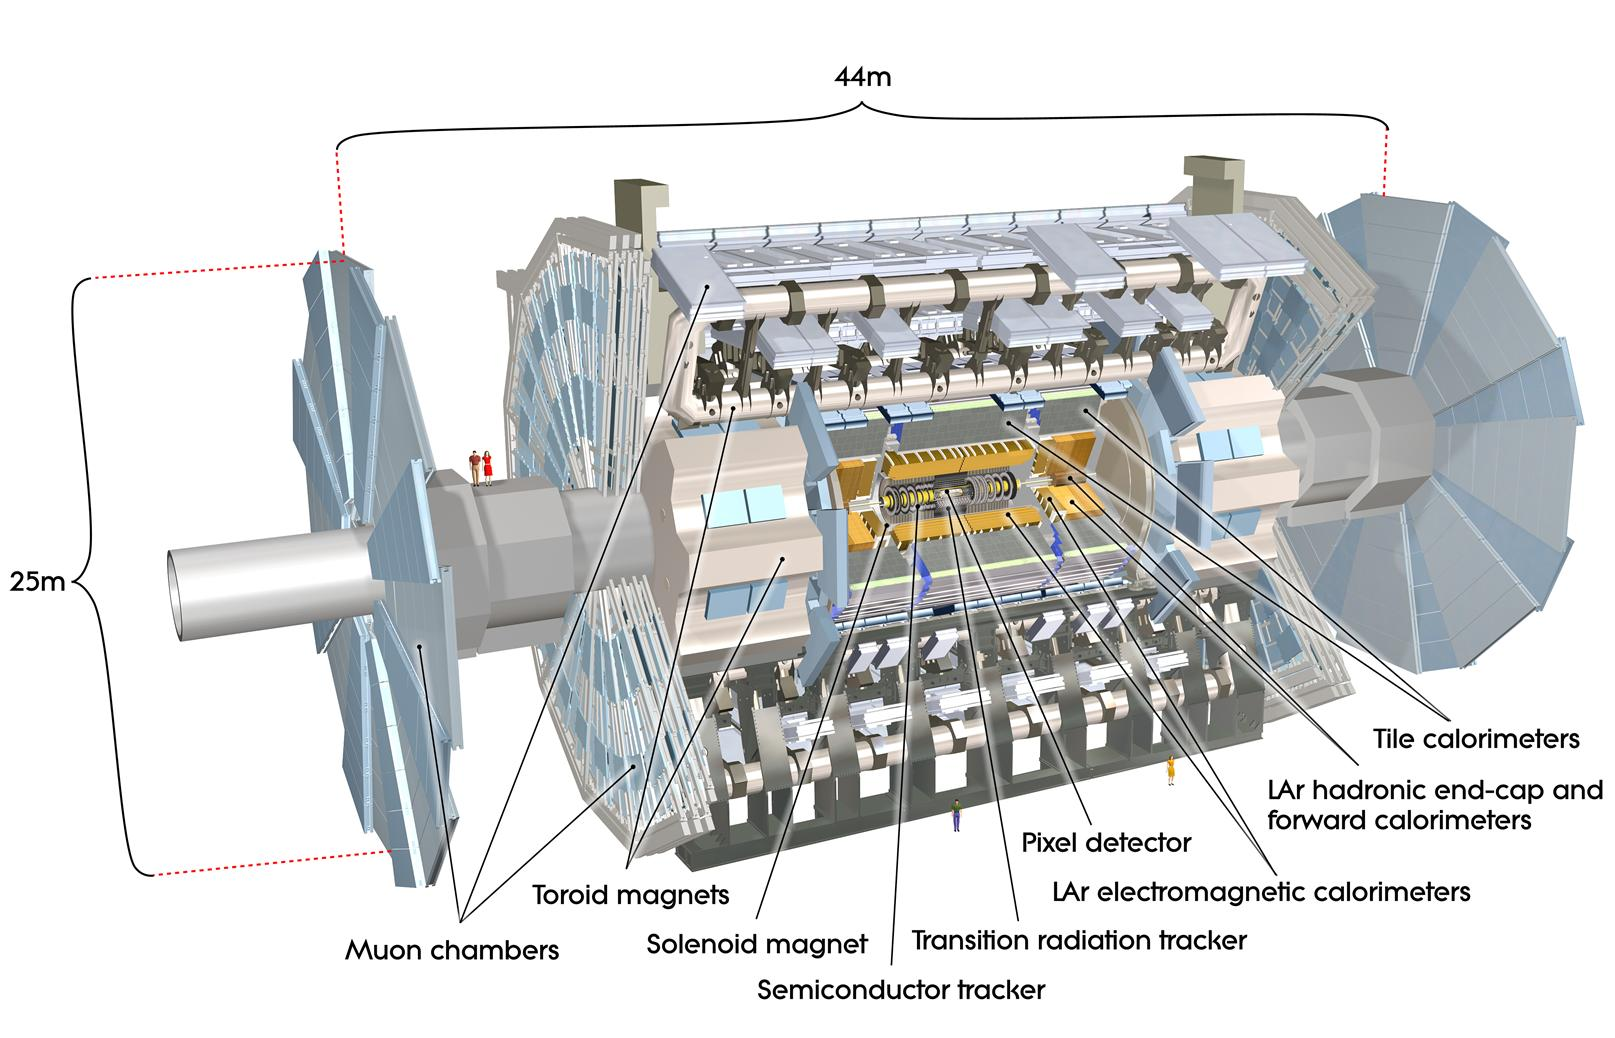
\includegraphics[width=0.8\textwidth]{figures/ATLAS_detector_0803012_01.jpg}\caption{Overview of the ATLAS detector showing all subsystems.} %https://cds.cern.ch/record/1095924 
\label{fig:atlas_detector}
\end{center}
\end{figure}

\subsection{Detector Geometry and Coordinate System}

ATLAS employs a right-handed coordinate system, illustrated in Figure~\ref{fig:atlas_coordinates}, with its origin at the nominal interaction point, chosen to reflect the detector's cylindrical geometry. The $z$-axis points along the beam direction toward the Jura mountains, the $x$-axis points toward the center of the LHC ring, and the $y$-axis points vertically upward. The azimuthal angle $\phi$ is measured in the $x$-$y$ plane from the positive $x$-axis, while the polar angle $\theta$ is measured from the positive $z$-axis.

\begin{figure}[!htb]
\begin{center}
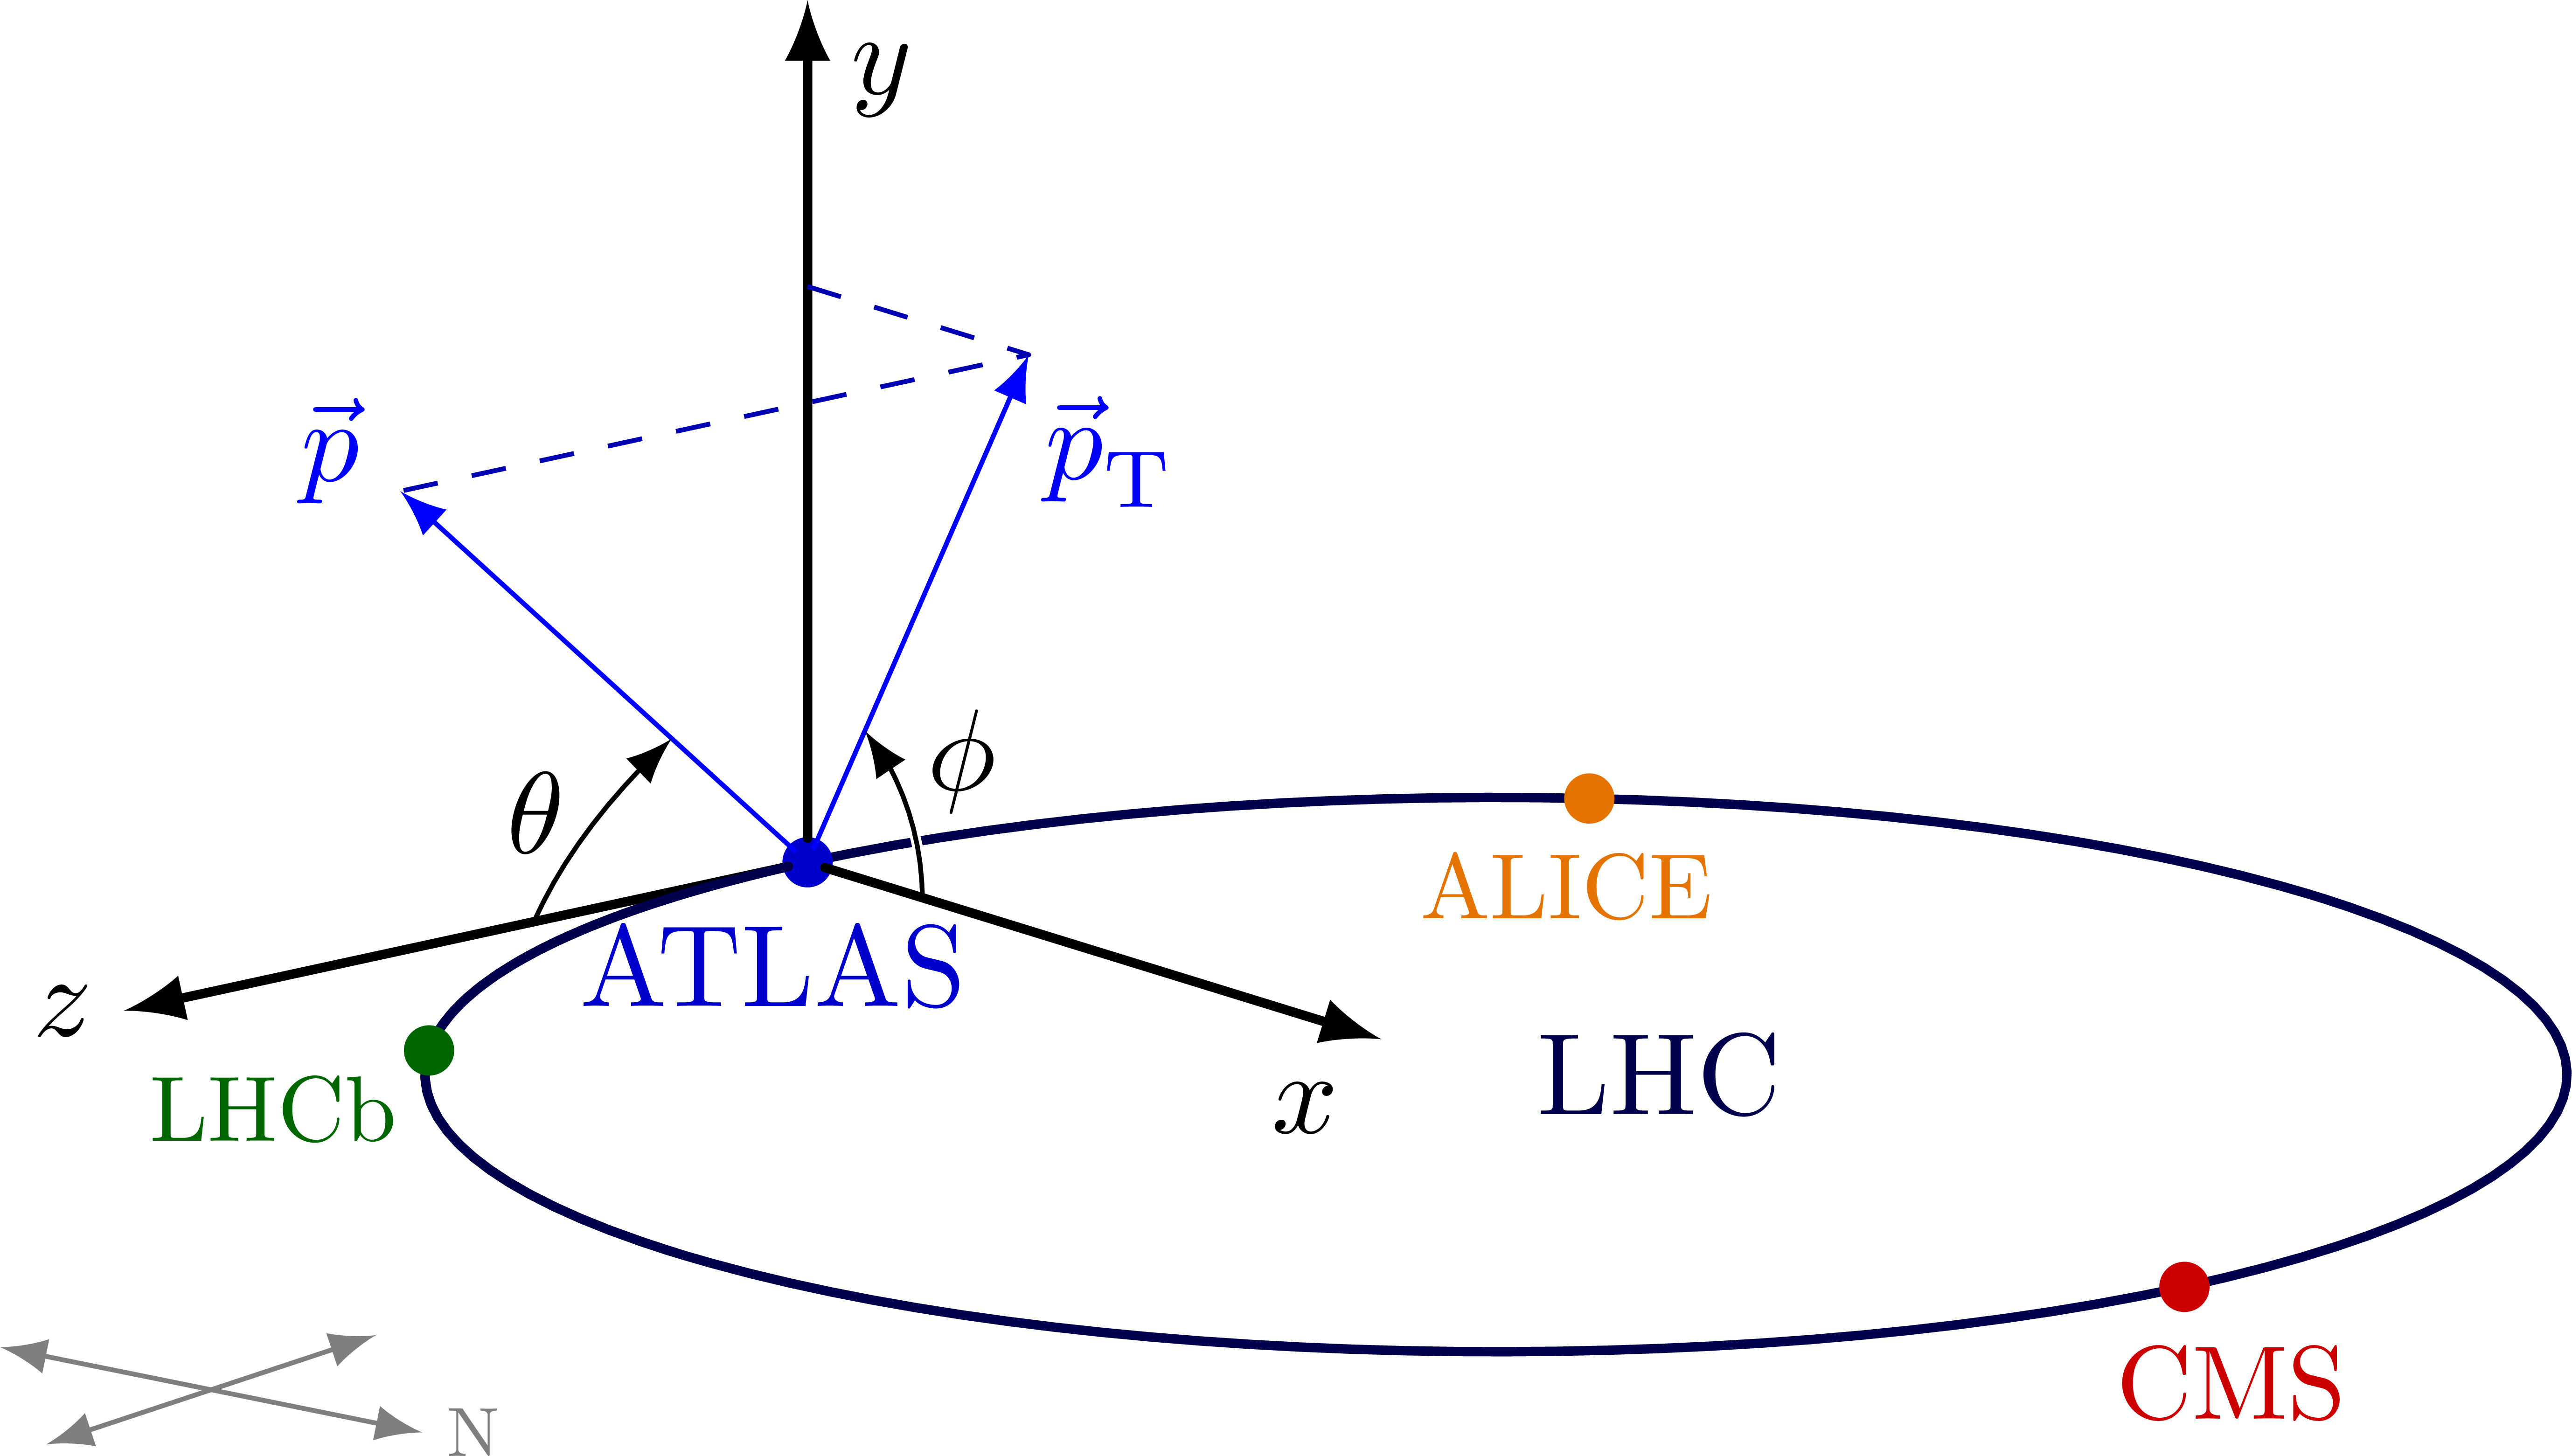
\includegraphics[width=0.8\textwidth]{figures/atlas_coordinate_system.png}\caption{Coordinate system of the ATLAS detector.} %https://tikz.net/axis3d_cms/
\label{fig:atlas_coordinates}
\end{center}
\end{figure}


In hadron collider physics, it is convenient to use the rapidity
\begin{equation}
y = \frac{1}{2} \ln\left(\frac{E + p_z}{E - p_z}\right),
\end{equation}
which transforms additively under longitudinal Lorentz boosts. For highly relativistic particles ($E \gg m$), the pseudorapidity
\begin{equation}
\eta = -\ln\left[\tan\left(\frac{\theta}{2}\right)\right]
\end{equation}
provides a good approximation to the rapidity and depends only on the polar angle.

The angular distance between two objects is typically expressed as
\begin{equation}
\Delta R = \sqrt{(\Delta\eta)^2 + (\Delta\phi)^2}.
\end{equation}

Kinematic variables are often expressed in terms of transverse quantities, because the longitudinal momentum of the colliding partons inside the protons is unknown. The transverse momentum $p_\text{T} = p\sin\theta$ and transverse energy $E_\text{T} = E\sin\theta$ are measured in the plane perpendicular to the beam axis.

The fundamental reason for the importance of these quantities lies in the principle of momentum conservation. While the total longitudinal momentum of the system is unknown, the total transverse momentum before the collision is zero. By the law of conservation of momentum, the vector sum of all transvere momenta of the final-state purticles must also be zero. This conservation principle allows for the calculation of the missing transverse momentum $\vec{p}_\text{T}^\text{miss}$ (with magnitude $E_\text{T}^\text{miss}$). $\vec{p}_\text{T}^\text{miss}$ is defined as the negative vector sum of all detected transverse momenta, indicating the presence of undetected particles such as neutrinos or other non-interacting particles.

\subsection{Inner Detector}

The Inner Detector (ID) is the innermost subdetector of ATLAS, surrounding the beam pipe and contained within a superconducting solenoid that provides a 2 T magnetic field. The ID extends from a radius of approximately 33 mm to 1,080 mm and covers a region of $|\eta| < 2.5$, providing precise tracking of charged particles through the measurement of their trajectories as they curve in the magnetic field.

The ID consists of three systems arranged in concentric cylinders:

\textbf{Pixel Detector:} The innermost tracking system, is positioned as the closest to the interaction point with the first layer (Insertable B-Layer, IBL) at only 33 mm from the beam axis. It's composed of four barrel layers and three end-cap disks per side. It employs approximately 92 million silicon pixels of typical size $50 \times 400$ $\mu$m$^{2}$ (and smaller $50 \times 250$ $\mu$m$^{2}$ pixels in the IBL), and measures 3D space points with high granularity, which is essential for precise vertex reconstruction and identification of $b$-quark jets through displaced vertex tagging.

\textbf{Semiconductor Tracker (SCT):} Surrounding the pixel detector, the SCT uses silicon microstrips with four double layers in the barrel and nine disks per end-cap. The SCT allows for 3D hit reconstruction from 6.3 million readout channels. Each particle typically crosses 8 strip layers. The SCT is designed to extend the tracking volume with a good balance between precision and coverage.

\textbf{Transition Radiation Tracker (TRT):} The outermost tracking component contains 298,000 drift tubes (straws) of 4 mm diameter filled with a Xe/CO$_2$/O$_2$ gas mixture. Particles typically traverse 36 straws. The TRT provides particle identification: when relativistic charged particles cross the polypropylene interfaces between the straws, they produce transition radiation photons, allowing for electron/pion discrimination.


The combined ID achieves a momentum resolution of $\sigma_{p_\text{T}}/p_T = 0.05\%\cdot p_\text{T}[\text{GeV}] \oplus 1\%$ and an impact parameter resolution of 10 $\mu$m for high-$p_\text{T}$ tracks.

\subsection{Calorimeters}

Located immediately outside the solenoid magned surrounding the ID, the ATLAS calorimeter system measures particle energies through total absorption in dense materials. The calorimeters are designed to contain the vast majority of the electromagnetic and hadronic showers while minimizing shower leakage to the muon system.

\textbf{Electromagnetic Calorimeter:} The Liquid Argon (LAr) electromagentic (EM) calorimeter is the primary detector for electrons and photons. Positioned at radii from 1.4 to 2.0 m in the barrel region, it uses liquid argon at 87 K as the active medium with lead absorbers arranged in an accordion geometry. This design provides full $\phi$ coverage without cracks and enables fast signal extraction. The EM calorimeter is divided into a barrel ($|\eta| < 1.475$), end-caps ($1.375 < |\eta| < 3.2$), and forward regions ($3.1 < |\eta| < 4.9$). It features three longitudinal samplings with varying granularity: strips of $\Delta\eta \times \Delta\phi = 0.003 \times 0.1$ in the first layer for $\pi^0/\gamma$ separation, $0.025 \times 0.025$ in the second layer containing most of the shower energy, and $0.05 \times 0.025$ in the third layer. A presampler detector in front of the accordion corrects for energy lost in upstream material. The total depth exceeds 22 radiation lengths ($X_0$) in the barrel. A key upgrade for Run 3 is the new LAr digital trigger electronics. This system significantly improves the granularity of the calorimeter information available at the L1 trigger, by approximately a factor of ten. This allows for a more precise and effective triggering on EM objects in the high pile-up environment.


\textbf{Hadronic Calorimeters:} Three distinct subsystems, each designed to cover a specific region of the detector, are used to measure the energy of hadrons and jets.


\textit{Tile Calorimeter}: Directly outside the EM calorimeter barrel, at radii 2.28-4.25 m, it covers $|\eta| < 1.7$. It is a sampling calorimeter that uses steel plates as the absorber material and scintillating tiles as the active medium. The system is divided into one central long barrel (LB) and two extended barrels (EB), each further segmented into 64 modules in the azimuthal angle. A plug detector, the Intermediate Tile Calorimeter (ITC), is located in the gap/crack region between the LB and EB. The ITC is desinged to measure the energy losses in the dead materials contained in the gap/crack region.

\textit{LAr Hadronic End-cap (HEC)}: Located behind the EM end-caps at $|z| > 4.3$ m, covering $1.5 < |\eta| < 3.2$. This system is also a sampling calorimeter, but with copper plates as the absorbers and liquid argon as the active medium. Its depth of approximately 10 interaction lengths ($\lambda$) is designed to contain most hadronic showers in this region.

\textit{LAr Forward Calorimeter (FCAL)}: Positioned at $|z| = 4.7$ m from the interaction point, covering $3.1 < |\eta| < 4.9$. It is specifically designed to operate in a region with very high particle flux. It uses dense absorber materials (copper for electromagnetic, tungsten for hadronic) and liquid argon as the active medium.

The combined calorimeter system achieves energy resolutions of $\sigma_E/E = 10\%/\sqrt{E[\text{GeV}]} \oplus 0.7\%$ for electromagnetic showers and $\sigma_E/E = 50\%/\sqrt{E[\text{GeV}]} \oplus 3\%$ for hadronic jets.





\subsection{Muon Spectrometer}

The Muon Spectrometer (MS) is the outermost layer of ATLAS, designed to identify and measure the momentum of muons. It extends from approximately 5 m radius in the barrel to 11 m, and reaches $|z| = 21.5$ m in the end-caps. The MS exploits the fact that muons above ~3 GeV are minimum ionizing particles that penetrate the calorimeters with minimal energy loss.

A toroidal magnetic field is generated in the MS by a system of eight rectangular coils in the barrel region (extending from 9.4 to 20.1 m in length) and two additional coils in the end-caps. The superconducting magnets generate magnetic fields of approximately 0.5 T in the barrel and 1 T in the end-caps. This field configuration bends muon trajectories in the $R$-$z$ plane in the barrel and $R$-$\phi$ plane in the end-caps.

For Run 3, the MS uses a combination of precision tracking and fast-response trigger chambers. The most significant upgrade for Run 3 was the replacement of the original Cathode Strip Chambers (CSCs) in the inner end-cap wheels with the New Small Wheels (NSW), which are specifically designed to handle the high background rates of the forward region.

The MS uses four complementary chamber technologies, organized into three distinct stations throughout the barrel and end-caps:


\textbf{Monitored Drift Tubes (MDT):} Provide precision tracking throughout most of the MS volume ($|\eta| < 2.7$). Each tube is 30 mm in diameter, operating with Ar/CO$_2$ gas at 3 bar, achieving 80 $\mu$m single-hit resolution. The chambers are positioned at approximately 5, 7.5, and 10 m radius in the barrel.

\textbf{Resistive Plate Chambers (RPC):} These chambers cover the barrel region ($|\eta| < 1.05$) in three doublet layers. They are fast-response detectors used for the muon trigger, providing a rapid signal with a 25 ns time resolution, and measuring the azimuthal coordinate. Each chamber consists of two resistive plates separated by a 2 mm gas gap. 

\textbf{Thin Gap Chambers (TGC):} Provide triggering in the end-cap region ($1.05 < |\eta| < 2.7$). These multiwire proportional chambers achieve 4 ns time resolution and measure both radial and azimuthal coordinates, with seven layers in the innermost station and three layers in the middle station.

\textbf{New Small Wheels (NSW):} The NSWs cover the region $1.3 < |\eta| < 2.7$, providing both precision tracking and L1 triggers. It consists of two detector technologies: Small-Strip Thin Gap Chambers (sTGC) for fast triggering and precise measurement of the muon's position; and Micromegas (MM) for high-precision trcking for momentum measurement.

The MS achieves a stand-alone momentum resolution of $\sigma_{p_T}/p_T \approx 10\%$ at 1 TeV, which improves to approximately 3\% when combined with ID measurements for muons traversing both systems.


\subsection{Trigger and Data Acquisition}

The ATLAS trigger and Data Acquisition (TDAQ) system is a two-level system that reduces the overwhelming 40 MHz bunch crossing rate to around 3 kHz for permanent storage. This ensures that only events with signatures of potentially interesting physics are saved for offline analysis.

\textbf{Level-1 Trigger (L1):} This is the first stage, hardware-based system, that makes a quick initial decision in just 2.5 $\mu$s. It uses information from the calorimeters and the MS to identify potential physics objects. For Run 3, the L1 trigger has been upgraded to use finer-granularity, digitalized calorimeter data, which allows for more precise object identification. This is further enhanced by the new L1 Topological (L1Topo) processors that apply simple topological selections, to reduce the rate more efficiently. The L1 trigger also integrates information from the NSW to improve the rejection of fake triggers. It reduces the event rate from 40 MHz down to a nominal 100 kHz and identifies Regions of Interest (RoI) for the next stage.

\textbf{High-Level Trigger (HLT):} This second and final stage is a software-based system that processes the events accepted by L1. It runs more sophisticated event reconstruction algorithms, but only on the data within the RoIs identified by L1. The HLT software has been redesigned to be multi-threaded for Run 3, allowing for a much more efficient use of the computing farm. The HLT selects events based on a trigger menu (a dynamic set of criteria and thresholds, optimized for each data-taking period), reducing the rate from 100 kHz to approximately 3kHz for permanent storage.

\textbf{Data Acquisition (DAQ):} The DAQ system manages the flow of data from the detector to the HLT and eventually to storage. When an event is accepted by the L1 trigger, the DAQ reads out the full high-resolution data from all subdetectors. A major upgrade for Run 3 is the new Front-End Link eXchange (FELIX) system. This is a high-throughput network that simplifies the data flow from the detector electronics to the HLT computing farm, making the entire DAQ system more scalable and flexible to handle the increased data volume and rates of Run 3.



\section{Object Identification and Reconstruction}

The identification and reconstruction of physics objects from detector signals is a fundamental step of all ATLAS physics analyses, allowing for the transformation of raw detector data into physics measurements. In Run 3, with average pile-up exceeding 50 interactions per bunch crossing, ATLAS has developed new algorithms that combine data from multiple detector subsystems to ensure that physics object reconstruction and analysis performance are maintained at or exceeding the levels of Run 2.

\subsection{Track and Vertex Reconstruction}

Track reconstruction begins with the formation of space points from hits in the ID silicon detectors. These space points are combined into track seeds, which are subsequently extended and fitted through the entire ID via a combinatorial Kalman filter. Track parameters are described by five quantities $(d_0, z_0, \phi, \theta, q/p)$ defined with respect to the beam spot, where $d_0$ and $z_0$ represent the transverse and longitudinal impact parameters, while $q/p$ denotes the charge-to-momentum ratio.

The primary inside-out tracking pass starts from three-hit seeds in the pixel detector and progressively adds compatible hits from outer layers. An ambiguity resolution algorithm removes duplicate and fake tracks by scoring candidates based on hit patterns, track $\chi^2$, and momentum. For Run 3, the tracking algorithms have been optimized to reduce fake track rates by more than 50\% while maintaining reconstruction efficiency above 99\% for tracks with $p_T > 1$ GeV.

Primary vertex reconstruction uses an iterative vertex finder that identifies the hard-scatter vertex among the multiple proton-proton interactions. The algorithm achieves longitudinal resolution better than 50 $\mu$m for vertices with more than 20 associated tracks, which is crucial for pile-up suppression and object-vertex association.

\subsection{Electron and Photon Reconstruction}

The reconstruction of electrons and photons in Run 3 utilizes dynamic, variable-size superclusters, replacing the fixed-size algorithm of previous runs. Reconstruction begins with topological clusters (topo-clusters) in the electromagnetic calorimeter, which are formed by grouping cells based on their signal significance, defined as the ratio of the cell's energy deposit to its expected noise ($E/\sigma_\text{noise}$). A cell can initiate a clusted (be a ``seed'') if its significance is greather than a set threshold, typically $4\sigma_\text{noise}$.

For electrons, reconstruction involves matching an ID track to a topological calorimeter cluster. To account for energy loss from bremsstrahlung, the track trajectory is refit using a specialized generalized Kalman Filter. The total energy of the electron is then measured by forming a supercluster, which aggregates the main energy deposit (the seed cluster) with smaller, nearby clusters created by bremsstrahlung photons. 

Photons are typically identified as electromagnetic clusters without a matching track. However, photons that convert into an $e^+e^-$ pair in the detector material are reconstructed using dedicated algorithms that find the secondary vertex ot the $e^+e^-$ pair.

Electron and photon identification employs multivariate techniques based on shower shapes, track quality, and transition radiation. The identification efficiencies in Run 3 show uncertainties reduced by 30-50\% compared to Run 2 results. The energy resolution achieved after calibration is on the order of 1-2\% for objects with $E_T > 25$ GeV.

\subsection{Muon Reconstruction}

Muon reconstruction combines measurements from the MS with information from the ID and calorimeters through two complementary strategies. The primary outside-in pass starts from track segments in the MS and matches them with ID tracks that extrapolate from the interaction point. These are then combined into a single, high-quality track, which is refit to account for energy loss.

An inside-out reconstruction chain complements this pass, and it's especially important for reconstructing muons with low $p_\text{T}$ or those in regions with limited MS coverage. This pass begins with a track found in the ID and attempts to extrapolate it outwards. It includes different types of recovered muons, such as ``segment-tagged'' muons, identified by a compatible MS segment, and ``calorimeter-tagged'' muons that leave a minimum-ionizing signature in the calorimeters.

Muon identification criteria range from ``Loose'' to ``Tight'' working points, and are optimized for different physics analyses. Large samples of $Z\to\mu\mu$ and $J/\psi\to\mu\mu$ decays are used for efficiency measurements of reconstruction and identification. The combined momentum resolution reaches $\sigma(p_T)/p_T \approx 2\%$ for muons with $p_T$ around 100 GeV.

\subsection{Jet Reconstruction and Particle Flow}

Starting from Run 3, the particle flow approach is the default method for jet reconstruction in ATLAS, representing a major improvement over traditional calorimeter-based methods. The particle flow algorithm's primary goal is to combine the most accurate measurements from all subdetectors to create a precise and complete reconstruction of each jet. It achieves this by using the highly accurate momentum measurement from the ID for charged particles and the calorimeter energy measurements for neutral particles, effectively avoiding the double-counting of energy.

The algorithm proceeds by first reconstructing tracks in the ID and extrapolating their trajectories to the calorimeter. These extrapolated tracks are then matched to topological clusters based on angular distance and the expected shower profile. For each matched track-cluster pair, the algorithm performs a cell-by-cell energy subtraction from the cluster. This subtraction removes the energy contribution of the charged particle, leaving behind the energy from neutral particles.

The remaining unsubtracted calorimeter deposits, which represent neutral particles (photons and neutral hadrons), are combined with the original charged particle tracks. This complete set of particle flow objects is then used as input to the anti-$k_t$ jet clustering algorithm. This method provides a more precise and complete description of the energy content of the jets.

The particle flow approach provides a 15-20\% improvement in jet energy resolution for jets with $p_\text{T}<70$ GeV compared to calorimeter-only reconstruction. This method is also more stable against the effects of high pile-up due to the precise vertex association of charged particles.

Jet energy scale calibration is performed in multiple stages, including pile-up subtraction, Monte Carlo-based calibration, and data-driven corrections.

\subsection{Heavy-Flavor Tagging}

The identification of jets containing $b$-hadrons (b-tagging) is crucial for many ATLAS physics analyses. It exploits the relatively long lifetime of $b$-hadrons ($c\tau \approx 450$ $\mu$m), which results in displaced decay vertices that are identified in the ID. For Run 3, ATLAS has moved to a new generation of tagging algorithms based on Graph Neural Networks (GNNs), with the GN2 algorithm becoming the new standard.

The GN2 algorithm uses a Transformer architecture to directly process individual track parameters and jet kinematics. In this approach, each track in a jet is treated as a node in a graph. The network analyzes a 23-dimensional feature vector for each track to predict the jet's flavor, while also identifying track origins and vertex associations. This advanced approach provides a significant performance increase over the previous tagger, DL1d. For example, at a 70\% b-tagging efficiency, GN2 improves light-jet rejection by approximately a factor of 2.5 and $c$-jet rejection by approximately a factor of 3.

The performance of b-tagging algorithms is calibrated using data-driven methods. This is tipically done by using large samples of $t\bar{t}$ events for $b$-jets and $D^{*+}$ mesons for $c$-jets.

\subsection{Tau Lepton Reconstruction}

Hadronic tau decays ($\tau_h$) are reconstructed from jets with $p_T > 10$ GeV and $|\eta| < 2.5$. For Run 3, ATLAS uses Recurrent Neural Networks (RNN) based algorithms for tau identification.

The RRN processes both individual tracks and calorimeter clusters to identify tau candidates and reject backgrounds. The RNN is particularly effective at handling the variable track multiplicity of tau decays (one or three charged particles). A dedicated energy calibration, which accounts for the unique shower shape of a tau, is then applied to the candidates using Boosted Regression Trees.

\subsection{Missing Transverse Momentum}

The missing transverse momentum $p_\text{T}^\text{miss}$, with magnitude $E_\text{T}^{\text{miss}}$, quantifies momentum imbalance in the transverse plane of the detector. A non-zero $E_\text{T}^{\text{miss}}$ indicates the presence of undetected particles, such as neutrinos or hypothetical BSM invisible particles, which do not interact with the detector. This measurement relies on the principle of momentum conservation: while the initial longitudinal momentum of the colliding partons is unknown, since the total transverse momentum of the initial colliding system is zero, the total transverse momentum of the final state must also be zero.

The $p_\text{T}^\text{miss}$ vector is calculated by summing the transverse momenta of all reconstructed particle flow objects. The algorithm uses the calibrated momenta of identified electrons, muons, photons and jets, as well as a ``soft term'' that accounts for low-$p_\text{T}$ particles and energy deposits not associated with any reconstructed object. 

The calculation vectorially sums transverse momenta of all particle flow objects, with identified electrons, muons, and photons replaced by their calibrated versions. A soft term accounts for low-$p_T$ particles not associated with reconstructed objects. The pile-up fit algorithm estimates and subtracts pile-up contributions based on spatial energy distributions across the calorimeter.

The $E_T^{\text{miss}}$ resolution scales approximately as $\sigma(E_T^{\text{miss}}) \approx 0.5\sqrt{\Sigma E_T}$ GeV$^{1/2}$, where $\Sigma E_T$ represents the scalar sum of transverse energies of all reconstructed objects. 